\section{Method}

This work follows four steps:

\begin{enumerate}
\item Data curation
\item Model training (with hyperparameter optimization)
\item Model validation
\item Model implementation in \Cyclus.
\end{enumerate}


First, we curated the
assembly information data for ease of use in training the model
(section \ref{unf}).
Second, we trained the dense neural network using Keras \cite{collet_keras_2015}
and Scikit-learn \cite{pedregosa_scikit-learn_2011}.
This workflow incorporated an outer loop to
search for the optimized set of neural network \textit{hyperparameters},
such as the number of hidden layers and nodes per layer.
Third, we used the model to predict the U.S. \gls{UNF}
inventory as specified in the \gls{UDB} and compare
\gls{UNF} inventory metrics such as fissile content
and decay heat. Lastly, we implemented the trained
model in \Cyclus by developing a reactor facility archetype
that transmutes fuel using the model.

The files used to generate and test the dense network
model are all on Github \footnote{https://github.com/jbae11/depletion\_rom}.
The raw data
is not available to the public.

\subsection{Training set}

In order to train an artificial neural network model, a significant database of
depletion data is needed that spans the potential
burnup and enrichment range in the reactor types involved
in the fuel cycle simulation.

Data from the \gls{UDB} was used to train the model 
based on burnup and enrichment. 

We simply used all the \gls{PWR} datasets in the \gls{UDB},
and the input values are only burnup and initial enrichment.
Ideally, the data should be generated with exact same reactor
parameters other than burnup and enrichment, such as lattice geometry.
However, the database is generated with varying
assembly geometries. 


\subsubsection{Unified Database}
\label{unf}
The \gls{UDB} is part of a larger engineering
analysis tool, the \gls{UNF-STANDARDS}, developed
by \gls{ORNL} \cite{peterson_used_2013}.  
The database provides a comprehensive, controlled
source of \gls{SNF} information, including
dry cask attributes, assembly data, economic attributes,
transportation infrastructure attributes, potential future
facility attributes, and federal government radioactive
waste attributes. 
The assembly-specific attributes include
initial enrichment, burnup, \gls{MTHM}, assembly 
type, and discharge date \cite{peterson_fuel_2015}. 
To generate this database, the authors used
irradiation and decay calculations using SCALE 
\cite{bowman_scale_2011}. The calculations were performed on each 
spent fuel assembly based on the previously mentioned 
parameters in the collected data to obtain mass, heat, 
and activity for each assembly \cite{peterson_additional_2017}. 
All the assemblies were modeled with conservative 
depletion parameters which result in the hardening of 
the neutron energy spectrum and an increased \gls{SNF} 
residual reactivity \cite{peterson_additional_2017}. 

Also, the irradiation history of the fuel is unspecified in the
database, which can be a source of deviation for short-lived isotopes.
With the unknown parameters (unknown irradiation history, varying
assembly models) and assumptions (conservative composition to
increase fuel reactivity), the database is far from ideal to use
as a training dataset for a depletion calculation model. However,
we chose this data set because it allows testing of model performance
through comparison of \gls{UNF}
inventory between a high-fidelity model and a model prediction for
varying burnup, enrichment, and discharge time.


We received the database through personal communication with
Dr. Kaushik Banerjee (ORNL).


\subsection{Data Curation}

We curated the raw \gls{UDB} datasets to generate
a cleaner training set. First, we only used the 
\gls{PWR} assemblies since \gls{BWR} \gls{UNF} assembly
calculation results can vary significantly with void fraction.
We also filtered out the
`very low' enrichment ($\leq$ 1.5) and
burnup ($\leq$ 10,000 MWd/MT)
assemblies to represent a more modern \gls{PWR} \gls{UNF}
assembly range. Figure \ref{fig:enr_bu} shows the
burnup and enrichment distribution of the assemblies in the
\gls{UDB}.


\begin{figure}
    \centering
    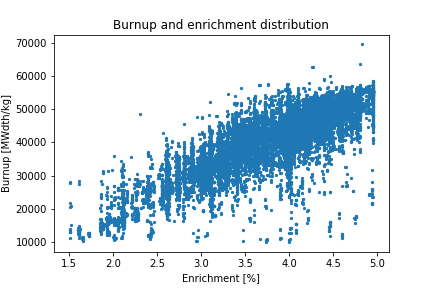
\includegraphics[width=\textwidth]{enr_bu.png}
    \caption{Burnup and enrichment distribution of train
             datasets curated from the \gls{UDB}.}
    \label{fig:enr_bu}
\end{figure}


Notably, since the SCALE calculations in the \gls{UDB} only track 60 isotopes,
3.5 weight percent of the \gls{UNF} is unaccounted for, on average. We
aggregate the isotopes not accounted for as a separate category. Lastly,
we processed the database so that the isotopic compositions are 
represented as weight \% normalized by initial uranium mass.
For every isotope \textit{i}:

\begin{equation}
x_i = \frac{m_i}{M_{initU}}
\end{equation}
where:
\begin{align}
x_i &= \text{Percent weight of isotope in depleted assembly}\\
m_i &= \text{Mass of isotope in depleted assembly in \gls{UDB}}\\
M_{initU} &= \text{Mass of initial uranium in assembly}
\end{align}


\subsection{Predictive Models for Fuel Depletion}

\gls{UNF} depleted composition prediction is complex
due to the varying relationship with the fuel parameters.
In figures \ref{fig:cs_137}, \ref{fig:pu_239}, and \ref{fig:u_235},
we observe the relationship between
burnup, enrichment, and isotopic composition.

We observed that, if the isotopic population is mainly determined by
the fission of initial uranium, a linear regression algorithm
can be used to predict the isotopic composition from burnup
(\textsuperscript{137}Cs shown in figure \ref{fig:cs_137}).
However, isotopes like \textsuperscript{239}Pu (figure \ref{fig:pu_239}) have multiple, conflicting creation
and destruction terms, making it harder to predict using a
linear regression algorithm. Also, the \textsuperscript{235}U (figure \ref{fig:u_235})
composition
depends on both burnup and enrichment, which can make it
hard to predict using a simple linear model.

Due to these complexities, we decided to train an artificial
dense neural network for our predictive model. We chose
Keras \cite{collet_keras_2015} to create and validate the model,
as well as scikit-learn \cite{pedregosa_scikit-learn_2011}
and pandas \cite{mckinney-proc-scipy-2010} for data processing and management.

\begin{figure}
    \centering
    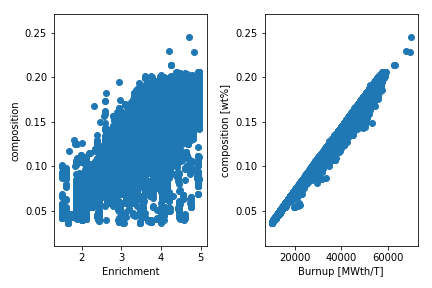
\includegraphics[width=\textwidth]{cs-137_sub.png}
    \caption{$^{137}Cs$ composition in a \gls{UNF} assembly
             varies linearly with assembly burnup.}
    \label{fig:cs_137}
\end{figure}

\begin{figure}
    \centering
    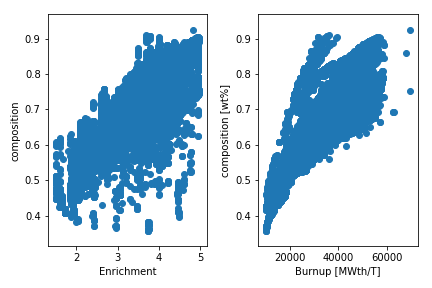
\includegraphics[width=\textwidth]{pu-239_sub.png}
    \caption{$^{239}Pu$ composition in a \gls{UNF} assembly
             is not linearly related to burnup, since it
             is affectex by multiple, conflicting creation
             and destruction terms}
    \label{fig:pu_239}
\end{figure}


\begin{figure}
    \centering
    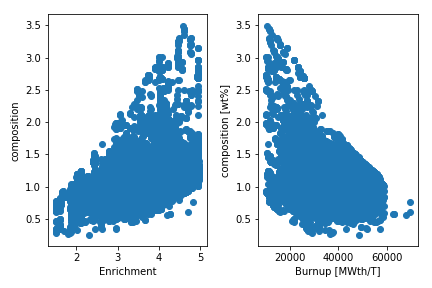
\includegraphics[width=\textwidth]{u-235_sub.png}
    \caption{$^{235}U$ composition in a \gls{UNF} assembly
             is somewhat proportional to both enrichment and
             burnup, but is difficult to predict using
             a simple linear regression algorithm.}
    \label{fig:u_235}
\end{figure}


\subsection{Training and Selecting Models}

The inputs (features) of the model are
burnup (MWd/MT) and initial enrichment (wt\% $^{235}U$).
The outputs (targets) of the model are
the composition (weight \%) of the 60 isotopes in the
depleted assembly.

With the curated dataset, we performed an outer loop
search to find the best-performing neural network
hyperparameter. First, we set aside 20 percent of the 
data for final model testing purposes. We used a three-fold
cross validation \cite{stone1974cross} on the remaining
dataset to
measure the average prediction error value. We
normalized the data using the \texttt{sklearn} MinMaxScaler
so that the range of input and output data was (0,1).

\begin{table}[h]
    \centering
    \begin{tabular}{lr}
        \hline
        Parameter & Values \\
        \hline
        Number of hidden layers & 1, \textbf{2}, 3, 4 \\
        Nodes per hidden layer & 4, 16, 32, 64, \textbf{128} \\
        Dropout rate & \textbf{0.0}, 0.2, 0.5 \\
        \hline
    \end{tabular}
    \caption{Table of hyperparameters tested
             for the neural network model. The bold
             numbers are the values we used for the final model.}
\end{table}


We selected the model with the smallest average error value
and exported the model as a Python
pickle file along with the dataset normalization objects and 
the list of isotopes. By exporting the trained model
as a self-contained file, the model can be used in any Python
application.


\subsection{Model Testing}

We tested the accuracy of the model by comparing
its \gls{UNF} composition prediction
in three different cases. First, we compared the
isotope-by-isotope prediction error of the model for an
assembly with a specific burnup and enrichment.
Second, we compared the waste characteristics of
an assembly to all assemblies. Third, we compared
the predicted total \gls{PWR} \gls{UNF} inventory with the
\gls{UDB}. The metric for error is calculated as
relative error percentage, $\epsilon$,
\begin{equation}
\epsilon = \frac{x_{data} - x_{model}}{x_{data}}
\end{equation}
where $x_{data}$ and $x_{model}$ are composition values
from the data and model, respectively.
This metric provides a fair assessment 
that is sensitive even to isotopes comprising a small
part of the total fuel mass.
Notably a large error percentage in the
prediction of these trace isotopes reflects a large
error with respect to weight \%, not necessarily a large absolute
mass difference.


We investigated the model accuracy with respect to fuel
cycle metrics such as activity and decay heat. The purpose
of this investigation is to see how this model can accurately
predict \gls{UNF} inventory profile in a \gls{NFC} simulator.

We compared parameters of the \gls{UNF} inventory
such as activity and decay heat, using the
\gls{PyNE} \cite{scopatz_pyne:_2012}. 

Ideally, the model should be tested against data
that is not part of the training data. However, given
that the purpose of this model is to allow accessible and
quick depletion calculation for
fuel cycle simulations, the model would suffice if
it predicts the dataset well. In other words, the
goal of the model is to be able to reproduce,
in a continuous manner, the range of fuel depletion
calculations in the database without access to the particular dataset
and to outperform simple interpolation with respect to accuracy.
This work
demonstrates a general approach for implementing
rapid depletion models in fuel cycle simulations.
To create depletion models for other reactor designs or depletion parameters,
one would simply change the dataset to a set of depletion calculations performed
for those specific reactor designs and operational parameters. 


\subsection{Model Implementation in \Cyclus}

The trained model is exported to a file
that can be plugged into external codes. Since \Cyclus
allows the developer
to design archetypes in python, we developed a Python-based reactor
module that behaves similarly to the \Cycamore reactor
but calculates depleted fuel composition using the
imported model instead of a recipe. The user defines a burnup
and enrichment
matrix for the reactor, and can even vary individual
assembly burnups. The rows are the number
%!%!%! instead of example, can you give a small matrix (display in math mode)
of batches, and the columns are the number of
assemblies in a batch. This reactor module is also
available on Github \footnote{https://github.com/jbae11/ann\_pwr}.

This sort of implementation can be done with
a recipe-based approach for modeling reactor depletion
if the user defines multiple
output recipes. However, the user can only define
the recipe of a batch.
Implementing this trained neural network model will allow the user to vary
burnup and enrichment for individual assemblies, as well
as vary fuel residence time and burnup with reactor
lifetime or simulation time. Such capability will be
useful in simulating the U.S. \gls{UNF} inventory in the future,
where the burnup of \gls{LWR} fuel will increase
with advanced fuel technology.